\documentclass{beamer}
\usepackage{tikz}
\usepackage{xcolor}
\usetikzlibrary{backgrounds,calc,positioning}
\usetikzlibrary{automata,positioning}
\usetheme{Antibes}
% \usetheme{Padova}
% \usetheme{boxes}
% \usetheme{Montpellier}

% \usefonttheme{serif}

\newcommand{\Buchi}{B{\"u}chi}
\newcommand{\trans}[1]{\overset{#1}{\rightarrow}}
\title{Simulation-based Inclusion Checking Algorithms for $\omega$-Languages}
% \subtitle{Using Beamer}
\author{Francesco Parolini}
\institute{Università degli Studi di Padova}
\date{23 July, 2020}
% 
\includegraphics[width=0.2\textwidth]{../img/logo-unipd.png}

\begin{document}
\begin{frame}
\titlepage
\end{frame}

% \section{The Language Inclusion Problem}
% \subsection{sub a}

%===============================================================================
\begin{frame}
\frametitle{Presentation}
\begin{itemize}
\item \textbf{Candidate:} Francesco Parolini
\item \textbf{Supervisor:} Prof. Francesco Ranzato
\item \textbf{Co-supervisor:} Prof. Pierre Ganty, IMDEA Software Institute, Madrid
\item \textbf{PhD. Student:} Kyveli Doveri, IMDEA Software Institute, Madrid
\end{itemize}
\end{frame}
%===============================================================================
\begin{frame}
\frametitle{The Language Inclusion Problem}
\begin{definition}[Language Inclusion Problem]
Let $L_1$ and $L_2$ be two languages.
The \textbf{language inclusion problem} consists in deciding whether
$L_1 \subseteq L_2$ holds or not.
\end{definition}

\begin{figure}[h]
	\centering
	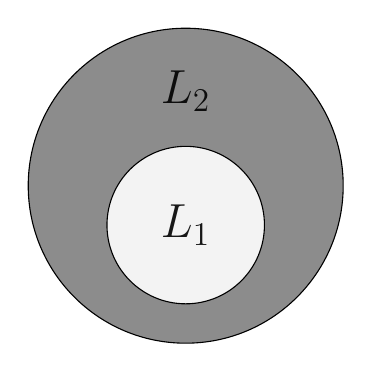
\begin{tikzpicture}
		\begin{scope} [fill opacity = .9]
			\draw[fill=gray, draw = black] (0,0) circle (2);
			\draw[fill=white, draw = black] (0,-0.5) circle (1);
			\node at (0,1.2) {\LARGE\textbf{$L_2$}};
			\node at (0,-0.5) {\LARGE\textbf{$L_1$}};
		\end{scope}
	\end{tikzpicture}
\end{figure}
\end{frame}


%===============================================================================
\begin{frame}
\frametitle{Characteristics}
% \begin{figure}[h]
%     \centering
%     \begin{tikzpicture}
%         \begin{scope} [fill opacity = .9]
%             \draw[fill=gray, draw = black] (0,0) circle (2);
%             \draw[fill=white, draw = black] (0,-0.5) circle (1);
%             \node at (0,1.2) {\LARGE\textbf{$L_2$}};
%             \node at (0,-0.5) {\LARGE\textbf{$L_1$}};
%         \end{scope}
%     \end{tikzpicture}
% \end{figure}

\begin{itemize}
\item Whether the problem is computable or not depends on the class of the languages
\item Also if it turns out to be computable, it is usually an hard problem
\end{itemize}

Applications
\begin{itemize}
% For example, in the automata-based approach to model-checking [18], both the system
% and the specification are represented as finite-state automata, and the model-checking
% problem reduces to testing whether any behavior of the system is allowed by the speci-
% fication, i.e., to a language inclusion problem.
\item Model checking
% Nei complilatori ovviamente il tokenizer viene implementato con un automa
\item Compilers construction
% Vedi il programma come un susseguirsi di configurazioni, da esperanza
\item Automata-based Verification
\end{itemize}
\end{frame}

%===============================================================================
\begin{frame}
\frametitle{$\omega$-languages}
\begin{definition}[$\omega$-language]
An \textbf{$\omega$-language} $L$ is a set of strings of \emph{infinite length} over some
alphabet $\Sigma$.
% alphabet $\Sigma$~\cite{cohen1977theory}.
\end{definition}

Examples of words of \textbf{infinite} length:
\[ abbb\cdots = ab^{\omega} \]
\[ babbaababab\cdots = babba(ba)^{\omega} \]
\end{frame}

%===============================================================================
\begin{frame}
\frametitle{\Buchi{} automata}
A \textbf{\Buchi{} automaton} is a tuple $\mathcal{B} = \langle Q, \delta, \{i\}, F\rangle$ \\
\begin{figure}[h]
\centering
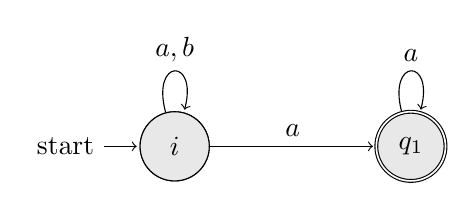
\begin{tikzpicture}[shorten >=1pt,node distance=3cm,auto]
  \tikzstyle{every state}=[fill={rgb:black,1;white,10}]
  \node[state] (q_0) {$i$};
  \node[state] (q_1) [right of=q_0]  {$q_1$};
  \pause
  \path[->]
  (q_0) edge [loop above] node {$a,b$} (q_0)
  (q_0) edge node {$a$} (q_1)
  (q_1) edge [loop above] node {$a$} (q_1)
  ;
  \pause
  \node[state,initial] (q_0) {$i$};
  \pause
  \node[state,accepting] (q_1) [right of=q_0]  {$q_1$};

\end{tikzpicture}
\end{figure}
\end{frame}

%===============================================================================
\begin{frame}
\frametitle{Traces}
A \textbf{trace} over the word $a_1a_2a_3\dots$:
\[ q_0 \trans{a_1} q_1 \trans{a_2} q_2 \trans{a_3} \cdots \]

\pause
A trace is \textbf{initial} if it starts in the initial state.

\pause
An \textbf{initial} trace over $(ab)^{\omega}$:
\begin{figure}[h]
\centering
\begin{tikzpicture}[shorten >=1pt,node distance=3cm,auto]
\tikzstyle{every state}=[fill={rgb:black,1;white,10}]
\node[state,initial] (q_0) {$i$};
\node[state,accepting] (q_1) [right of=q_0]  {$q_1$};
\path[->]
(q_0) edge [loop above] node {$a$,$b$} (q_0)
(q_0) edge node {$a$} (q_1)
(q_1) edge [loop above] node {$a$} (q_1)
;
\pause
\node[state] (q_0) {\textcolor{red}{$i$}};
\node at (-1,-2)  {\Large$i$};
\pause
\node[state] (q_0) {$i$};
\path[->] (q_0) edge [loop above] node {\textcolor{red}{$a$},$b$} (q_0) ;
\node at (-0.6,-1.9)  {\Large$\overset{a}{\rightarrow}$};
\pause
\path[->] (q_0) edge [loop above] node {$a$,$b$} (q_0) ;
\node[state] (q_0) {\textcolor{red}{$i$}};
\node at (-0.2,-2)  {\Large$i$};
\pause
\node[state] (q_0) {$i$};
\path[->] (q_0) edge [loop above] node {$a$,\textcolor{red}{$b$}} (q_0) ;
\node at (0.2,-1.85)  {\Large$\overset{b}{\rightarrow}$};

\pause
\path[->] (q_0) edge [loop above] node {$a$,$b$} (q_0) ;
\node[state] (q_0) {\textcolor{red}{$i$}};
\node at (0.6,-2)  {\Large$i$};
\pause
\node[state] (q_0) {$i$};
\path[->] (q_0) edge [loop above] node {\textcolor{red}{$a$},$b$} (q_0) ;
\node at (1,-1.9)  {\Large$\overset{a}{\rightarrow}$};
\pause
\path[->] (q_0) edge [loop above] node {$a$,$b$} (q_0) ;
\node[state] (q_0) {\textcolor{red}{$i$}};
\node at (1.4,-2)  {\Large$i$};
\pause
\node[state] (q_0) {$i$};
\path[->] (q_0) edge [loop above] node {$a$,\textcolor{red}{$b$}} (q_0) ;
\node at (2.2,-1.85)  {\Large$\overset{b}{\rightarrow}\cdots$};
\end{tikzpicture}
\end{figure}
\end{frame}

%===============================================================================
\begin{frame}
\frametitle{Traces}
A \textbf{fair} trace over the word $a_1a_2a_3\dots$:
\[ q_0 \trans{a_1} \textcolor{red}{q_f} \trans{a_2} q_3 \trans{a_3} \cdots \trans{a_i}
\textcolor{red}{q_f} \trans{a_{i+1}} \cdots \trans{a_j} \textcolor{red}{q_f} \trans{a_{j+1}} \cdots\]

\pause
An \textbf{initial} and \textbf{fair} trace over $aba ^{\omega}$:
\begin{figure}[h]
\centering
\begin{tikzpicture}[shorten >=1pt,node distance=3cm,auto]
  \tikzstyle{every state}=[fill={rgb:black,1;white,10}]
  \node[state,initial] (q_0) {$i$};
  \node[state,accepting] (q_1) [right of=q_0]  {$q_1$};
  \path[->]
  (q_0) edge [loop above] node {$a$,$b$} (q_0)
  (q_0) edge node {$a$} (q_1)
  (q_1) edge [loop above] node {$a$} (q_1)
  ;
  \pause
  \node[state] (q_0) {\textcolor{red}{$i$}};
  \node at (-1,-2)  {\Large$i$};
  \pause
  \node[state] (q_0) {$i$};
  \path[->] (q_0) edge [loop above] node {\textcolor{red}{$a$},$b$} (q_0) ;
  \node at (-0.6,-1.9)  {\Large$\overset{a}{\rightarrow}$};
  \pause
  \path[->] (q_0) edge [loop above] node {$a$,$b$} (q_0) ;
  \node[state] (q_0) {\textcolor{red}{$i$}};
  \node at (-0.2,-2)  {\Large$i$};
  \pause
  \node[state] (q_0) {$i$};
  \path[->] (q_0) edge [loop above] node {$a$,\textcolor{red}{$b$}} (q_0) ;
  \node at (0.2,-1.85)  {\Large$\overset{b}{\rightarrow}$};
  \pause
  \path[->] (q_0) edge [loop above] node {$a$,$b$} (q_0) ;
  \node[state] (q_0) {\textcolor{red}{$i$}};
  \node at (0.6,-2)  {\Large$i$};
  \pause
  \node[state] (q_0) {$i$};
  \path[->] (q_0) edge node {\textcolor{red}{$a$}} (q_1) ;
  \node at (1,-1.9)  {\Large$\overset{a}{\rightarrow}$};
  \pause
  \path[->] (q_0) edge node {$a$} (q_1) ;
  \node[state,accepting] (q_1) [right of=q_0]  {\textcolor{red}{$q_1$}};
  \node at (1.5,-2.05)  {\Large$q_1$};
  \pause
  \node[state,accepting] (q_1) [right of=q_0]  {$q_1$};
  \path[->] (q_1) edge [loop above] node {\textcolor{red}{$a$}} (q_1);
  \node at (2,-1.9)  {\Large$\overset{a}{\rightarrow}$};
  \pause
  \path[->] (q_1) edge [loop above] node {$a$} (q_1);
  \node[state,accepting] (q_1) [right of=q_0]  {\textcolor{red}{$q_1$}};
  \node at (2.5,-2.05)  {\Large$q_1$};
  \pause
  \node[state,accepting] (q_1) [right of=q_0]  {$q_1$};
  \path[->] (q_1) edge [loop above] node {\textcolor{red}{$a$}} (q_1);
  \node at (3.4,-1.9)  {\Large$\overset{a}{\rightarrow}\cdots$};
\end{tikzpicture}
\end{figure}
\end{frame}

%===============================================================================
\begin{frame}
The \emph{language recognized by a \Buchi{} automaton} $\mathcal{B}$ is:
\[ \mathcal{L}(\mathcal{B}) = \{w \;|\; \textrm{there is an initial and fair trace over $w$} \} \]

\begin{example}
\frametitle{The language of a \Buchi{} automaton}
\begin{figure}[h]
\centering
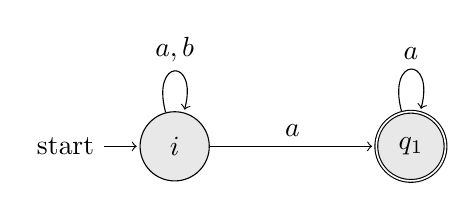
\begin{tikzpicture}[shorten >=1pt,node distance=3cm,auto]
  \tikzstyle{every state}=[fill={rgb:black,1;white,10}]
  \node[state,initial] (q_0) {$i$};
  \node[state,accepting] (q_1) [right of=q_0]  {$q_1$};
  \path[->]
  (q_0) edge [loop above] node {$a,b$} (q_0)
  (q_0) edge node {$a$} (q_1)
  (q_1) edge [loop above] node {$a$} (q_1)
  ;
\end{tikzpicture}
\end{figure}
\[ \mathcal{L}(\mathcal{B}) = \{a ^{\omega}, b a ^{\omega}, ab a^{\omega}, bb a^{\omega}, \dots\} = (a + b)^* a ^{\omega} \]
\end{example}

\end{frame}

\begin{frame}
\frametitle{$\omega-$regular languages}
\begin{definition}[$\omega$-regular language]
The class of languages recognized by \Buchi{} automata is called
\textbf{$\omega$-regular languages}.
\end{definition}
Applications
\begin{itemize}
% For example, in the automata-based approach to model-checking [18], both the system
% and the specification are represented as finite-state automata, and the model-checking
% problem reduces to testing whether any behavior of the system is allowed by the speci-
% fication, i.e., to a language inclusion problem.
\item Model checking
% hoffman and chen
\item Type systems
% \item Reasoning for logical theories
\end{itemize}
\end{frame}

%===============================================================================
\begin{frame}
\frametitle{Deciding the Language Inclusion}
\begin{itemize}
\item Languages are \textbf{not finite}, we can't just compare them
\pause
\item \textbf{Abstract Interpretation:}
    \begin{itemize}
    \item Static program analysis
    \item Giving up precision for computability
    \end{itemize}
\end{itemize}
\end{frame}

%===============================================================================
\begin{frame}
\frametitle{Deciding the Language Inclusion}
We started from the ``Doveri-Ganty'' framework for checking the language inclusion,
which relies on \emph{Abstract Interpretation} techniques.

\begin{figure}[h]
	\centering
	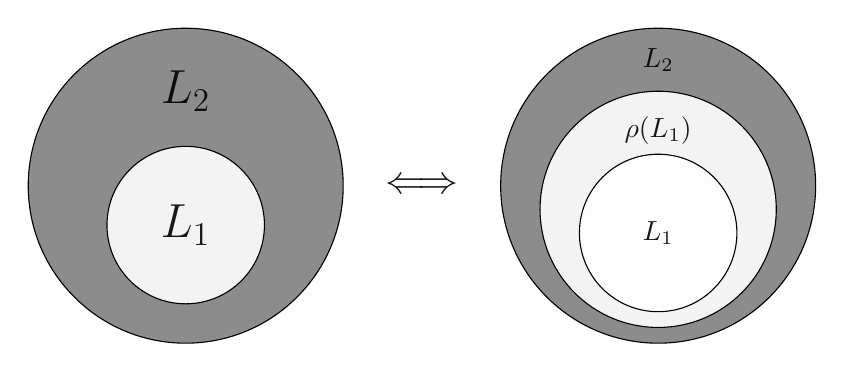
\begin{tikzpicture}
		\begin{scope} [fill opacity = .9]
			\draw[fill=gray, draw = black] (0,0) circle (2);
			\draw[fill=white, draw = black] (0,-0.5) circle (1);
			\node at (0,1.2) {\LARGE\textbf{$L_2$}};
			\node at (0,-0.5) {\LARGE\textbf{$L_1$}};

			\draw[fill=gray, draw = black] (6,0) circle (2);
			\draw[fill=white, draw = black] (6,-0.3) circle (1.5);
			\draw[fill=white, draw = black] (6,-0.6) circle (1);
			\node at (6,1.6)  {\textbf{$L_2$}};
			\node at (6,0.7)  {\textbf{$\rho(L_1)$}};
			\node at (6,-0.6) {\textbf{$L_1$}};
			\node at (3,0) {\Large\textbf{$\Longleftrightarrow$}};
		\end{scope}
	\end{tikzpicture}
\end{figure}
\end{frame}



%===============================================================================
\begin{frame}
\frametitle{Details}
A \textbf{ultimately periodic} word:
\[ abc(de)^{\omega} \]
We define:
% \[ UP(L) = \{uv ^{\omega} \in \Sigma^* \times \Sigma^+ \;|\; uv ^{\omega} \in L\} \]
\[ I_{L} \overset{\triangle}{=} \{ (u,v) \;|\; uv ^{\omega} \in L\} \]
Then, one key observation is:
\begin{equation*}
\begin{split}
L_1 \subseteq L_2 & \Longleftrightarrow I_{L_1} \subseteq I_{L_2}
\end{split}
\end{equation*}

Let $\leq_1, \leq_2$ be two \textbf{preorders} on words.
\[ \rho_{\leq_1 \times \leq_2}(I_L) \overset{\triangle}{=} \{(s,t) \;|\; \exists (u,v) \in I_L, u \leq_1 s \; \wedge \; v \leq_2 t\} \]
\end{frame}


%===============================================================================
\begin{frame}
Let $\leq_1, \leq_2$ be two preorders on words that
meet a list of requirements related to \textbf{computability} and \textbf{completeness}.
\[ L_1 \subseteq L_2 \Longleftrightarrow \rho_{\leq_1 \times \leq_2}(I_{L_1}) \subseteq I_{L_2}  \]

\begin{figure}[h]
	\centering
	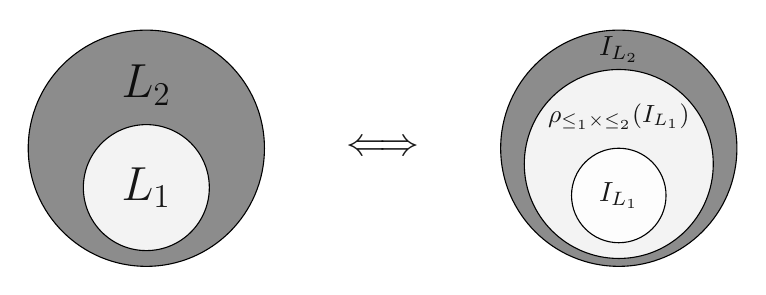
\begin{tikzpicture}
		\begin{scope} [fill opacity = .9]
			\draw[fill=gray, draw = black] (0,0) circle (1.5);
			\draw[fill=white, draw = black] (0,-0.5) circle (0.8);
			\node at (0,0.8) {\LARGE\textbf{$L_2$}};
			\node at (0,-0.5) {\LARGE\textbf{$L_1$}};

			\draw[fill=gray, draw = black] (6,0) circle (1.5);
			\draw[fill=white, draw = black] (6,-0.2) circle (1.2);
			\draw[fill=white, draw = black] (6,-0.6) circle (0.6);
			\node at (6,1.25)  {\textbf{$I_{L_2}$}};
			\node at (6,0.4)  {\small\textbf{$\rho_{\leq_1 \times \leq_2}(I_{L_1})$}};
			\node at (6,-0.6) {\textbf{$I_{L_1}$}};
			\node at (3,0) {\Large\textbf{$\Longleftrightarrow$}};
		\end{scope}
	\end{tikzpicture}
\end{figure}

% \textbf{Completeness:} Why?

\textbf{Observation:} usually when abstracting one object we gain decidability,
but here the abstraction goes from one infinite set ($I_{L_1}$) to another
infinite set... Why?
\end{frame}



%===============================================================================
\begin{frame}
\frametitle{Gaining decidability}
We can extract from the abstraction $\rho_{\leq_1 \times \leq_2}(I_{L_1})$
a \textbf{finite} set, say $T$, such that:
\[ L_1 \subseteq L_2 \Longleftrightarrow \forall (u,v) \in T, uv^{\omega} \in L_2\]

% They also give an algorithm, \texttt{BAInc}, that computes the set $T$ using the two preorders
% $\leq_1$ and $\leq_2$, then checking whether
% $\forall (u,v) \in T, uv ^{\omega} \in L_2$, deciding if $L_1 \subseteq L_2$
% holds or not.

\begin{figure}[h]
	\centering
	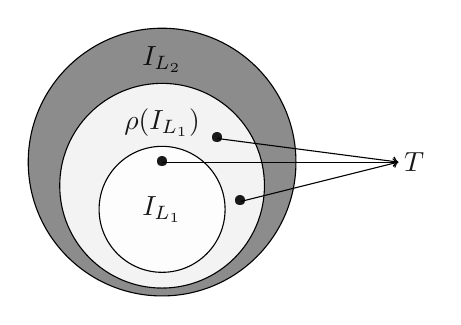
\begin{tikzpicture}
		\begin{scope} [fill opacity = .9]
			% \draw[fill=gray, draw = black] (0,0) circle (1.5);
			% \draw[fill=white, draw = black] (0,-0.5) circle (0.8);
			% \node at (0,0.8) {\LARGE\textbf{$I_{L_2}$}};
			% \node at (0,-0.5) {\LARGE\textbf{$I_{L_1}$}};

			\draw[fill=gray, draw = black] (6,0) circle (1.7);
			\draw[fill=white, draw = black] (6,-0.3) circle (1.3);
			\draw[fill=white, draw = black] (6,-0.6) circle (0.8);
			\node at (6,1.3)  {\textbf{$I_{L_2}$}};
			\node at (6,0.5)  {\textbf{$\rho(I_{L_1})$}};
			\node at (6,-0.6) {\textbf{$I_{L_1}$}};
            \draw (6,0) node {\textbullet};
            \draw[-> ] (6,0) -- (9,0);
            \draw (6.7,0.3) node {\textbullet};
            \draw[-> ] (6.7,0.3) -- (9,0);
            \draw (7,-0.5) node {\textbullet};
            \draw[-> ] (7,-0.5) -- (9,0);

            \draw (9.2,0) node {$T$};
		\end{scope}
	\end{tikzpicture}
\end{figure}

\end{frame}



%===============================================================================
\begin{frame}
\frametitle{Algorithm to solve $L_1 \subseteq L_2$}
% Summarizing, \texttt{BAInc} is one algorithm that is parametrized by a pair
% of preorders $(\leq_1, \leq_2)$ and solves the language inclusion problem.
% The pair of preorders have to meet a list of requirements related to computability
% and completeness.
% They also define two families of preorders that meet the criteria:
\begin{itemize}
\item They give \texttt{BAInc}, algorithm to solve $L_1 \subseteq L_2$
    \begin{enumerate}
    \item Computes $T$
    \item Checks if $\forall (u,v) \in T, uv ^{\omega} \in L_2$
    \end{enumerate}
\item \texttt{BAInc} is parametrized by $\leq_1, \leq_2$
\end{itemize}

\begin{figure}[h]
\centering
\begin{tikzpicture}[shorten >=1pt,node distance=3cm,auto]
  \tikzstyle{every state}=[fill={rgb:black,1;white,10}]
  \node (0) {$\leq^2_{\mathcal{B}}$};
  \node (1) [right of=0]{$\leq^1_{\mathcal{B}}$};
  \node (2) [right of=1]{$\leq^r_{\mathcal{B}}$};
  \node (8)  [below of=0] {$\leq^2_{L}$};
  \node (9)  [right of=8]{$\leq^1_{L}$};
  \node (10) [right of=9]{$\leq^r_{L}$};
  \path[->]
  (0) edge node {} (1)
  (0) edge node {} (8)
  (1) edge node {} (2)
  (1) edge node {} (9)
  (8) edge node {} (9)
  (9) edge node {} (10)
  (2) edge node {} (10)
  ;
\end{tikzpicture}
\end{figure}

\pause
\textbf{My task:} to define new preorders $\leq_1, \leq_2$
\end{frame}

%===============================================================================
\begin{frame}
\frametitle{Simulations}
\begin{itemize}
\item Behavioural relations
\item Intuitively, one state is simulated by another if the second can match all the moves of the first
\item Fundamental in Process Calculi
\item There are many known algorithms to compute simulations
\end{itemize}
\end{frame}

%===============================================================================
\begin{frame}
\frametitle{The Game of Simulation}

\begin{figure}[h]
\centering
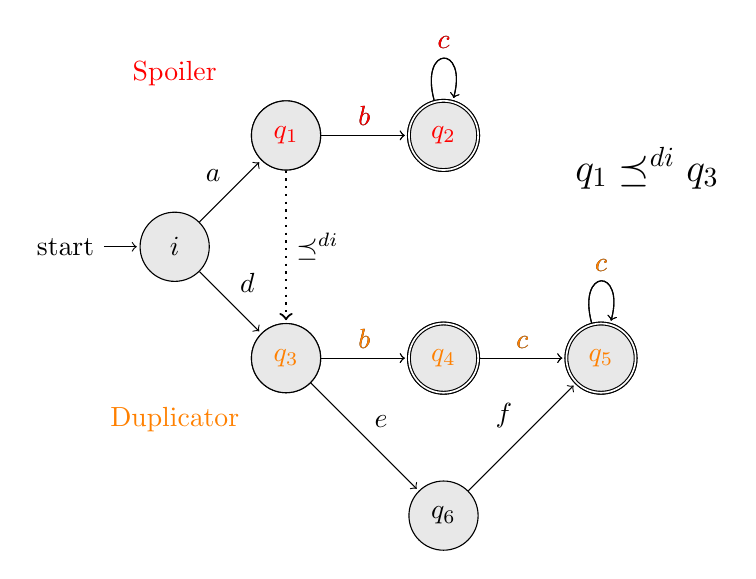
\begin{tikzpicture}[shorten >=1pt,node distance=2cm,auto]
  \tikzstyle{every state}=[fill={rgb:black,1;white,10}]
  \node[state,initial] (q_0) {$i$};
  \node[state] (q_1) [above right of=q_0]  {$q_1$};
  \node[state,accepting] (q_2) [right of=q_1]  {$q_2$};
  \node[state] (q_3) [below right of=q_0]  {$q_3$};
  \node[state,accepting] (q_4) [right of=q_3]  {$q_4$};
  \node[state,accepting] (q_5) [right of=q_4]  {$q_5$};
  \node[state] (q_6) [below of=q_4]  {$q_6$};
  \path[->]
  (q_0) edge node {$a$} (q_1)
  (q_0) edge node {$d$} (q_3)
  (q_1) edge node {$b$} (q_2)
  (q_3) edge node {$b$} (q_4)
  (q_3) edge node {$e$} (q_6)
  (q_6) edge node {$f$} (q_5)
  (q_4) edge node {$c$} (q_5)
  (q_2) edge [loop above] node {$c$} (q_2)
  (q_5) edge [loop above] node {$c$} (q_5)
  ;
    \pause
  \draw (0,2.2) node {\textcolor{red}{Spoiler}};
  \draw (0,-2.2) node {\textcolor{orange}{Duplicator}};
    \node[state] (q_1) [above right of=q_0]  {\textcolor{red}{$q_1$}};
  \node[state] (q_3) [below right of=q_0]  {\textcolor{orange}{$q_3$}};

  \pause
\path[->]
  (q_1) edge node {\textcolor{red}{$b$}} (q_2)
  ;

  \pause
  \node[state, accepting] (q_2) [right of=q_1]  {\textcolor{red}{$q_2$}};

  \pause
\path[->]
  (q_3) edge node {\textcolor{orange}{$b$}} (q_4)
  ;

  \pause
  \node[state, accepting] (q_4) [right of=q_3]  {\textcolor{orange}{$q_4$}};

  \pause
\path[->]
  (q_2) edge [loop above] node {\textcolor{red}{$c$}} (q_2)
  ;

  \pause
\path[->]
  (q_4) edge node {\textcolor{orange}{$c$}} (q_5)
  ;

    \pause
  \node[state, accepting] (q_5) [right of=q_4]  {\textcolor{orange}{$q_5$}};

      \pause
\path[->] (q_5) edge [loop above] node {\textcolor{orange}{$c$}} (q_5) ;


    \pause
  \draw (6,1) node {\Large$q_1 \preceq^{di} q_3 $};
\path[->, dotted, thick] (q_1) edge node {$\preceq^{di}$} (q_3) ;


\end{tikzpicture}
\end{figure}
\end{frame}

%===============================================================================
\begin{frame}
\frametitle{My work}
I started from:
\begin{equation*}
\begin{split}
u \sqsubseteq_{\mathcal{B}}^r v \Longleftrightarrow \; & \textrm{\textbf{for each} state $p$
such that $i \overset{u}{\rightsquigarrow} p$,} \\
& \textrm{\textbf{exists} a state $q$ such that $i \overset{v}{\rightsquigarrow} q$ and $p \preceq^{di} q$}
\end{split}
\end{equation*}

\begin{figure}[h]
\centering
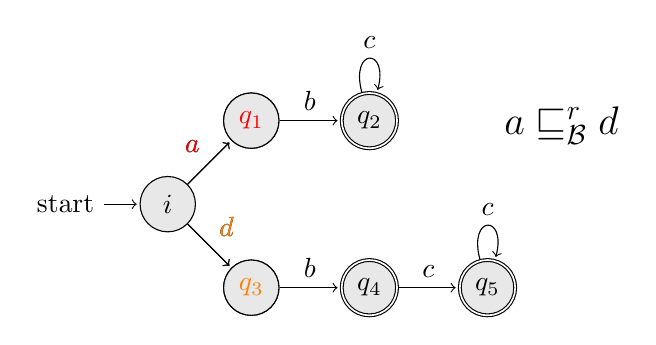
\begin{tikzpicture}[shorten >=1pt,node distance=1.5cm,auto]
  \tikzstyle{every state}=[fill={rgb:black,1;white,10}]
  \node[state,initial,inner sep=1pt,minimum size=20pt] (q_0) {$i$};
  \node[state,inner sep=1pt,minimum size=20pt] (q_1) [above right of=q_0]  {$q_1$};
  \node[state,accepting,inner sep=1pt,minimum size=20pt] (q_2) [right of=q_1]  {$q_2$};
  \node[state,inner sep=1pt,minimum size=20pt] (q_3) [below right of=q_0]  {$q_3$};
  \node[state,inner sep=1pt,minimum size=20pt,accepting] (q_4) [right of=q_3]  {$q_4$};
  \node[state,inner sep=1pt,minimum size=20pt,accepting] (q_5) [right of=q_4]  {$q_5$};
  \path[->]
  (q_0) edge node {$a$} (q_1)
  (q_0) edge node {$d$} (q_3)
  (q_1) edge node {$b$} (q_2)
  (q_3) edge node {$b$} (q_4)
  (q_4) edge node {$c$} (q_5)
  (q_2) edge [loop above] node {$c$} (q_2)
  (q_5) edge [loop above] node {$c$} (q_5)
  ;
    \pause
  \path[->]   (q_0) edge node {\textcolor{red}{$a$}} (q_1) ;
    \node[state,inner sep=1pt,minimum size=20pt] (q_1) [above right of=q_0]  {\textcolor{red}{$q_1$}};

    \pause
  \path[->]   (q_0) edge node {\textcolor{orange}{$d$}} (q_3) ;
  \node[state,inner sep=1pt,minimum size=20pt] (q_3) [below right of=q_0]  {\textcolor{orange}{$q_3$}};
  \pause
  \draw (5,1) node {\Large$a \sqsubseteq^r_{\mathcal{B}}d $};
\end{tikzpicture}
\end{figure}

\end{frame}


%===============================================================================
\begin{frame}
\frametitle{New preorders}

Generalization using \textbf{different simulations}:
\begin{itemize}
\Large\item $\sqsubseteq_{\mathcal{B}}^{de,r}$
\end{itemize}
\begin{figure}[h]
\centering
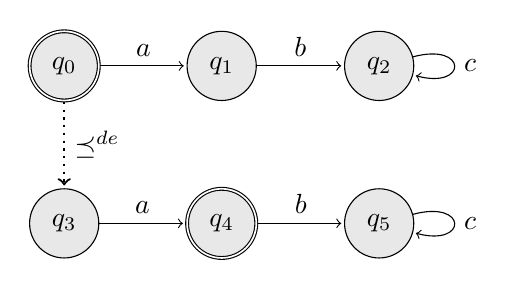
\begin{tikzpicture}[shorten >=1pt,node distance=2cm,auto]
  \tikzstyle{every state}=[fill={rgb:black,1;white,10}]
  \node[state,accepting] (q_0) {$q_0$};
  \node[state] (q_1) [right of=q_0]  {$q_1$};
  \node[state] (q_2) [right of=q_1]  {$q_2$};
  \node[state] (q_3) [below of=q_0] {$q_3$};
  \node[state,accepting] (q_4) [right of=q_3]  {$q_4$};
  \node[state] (q_5) [right of=q_4]  {$q_5$};
  \path[->]
  (q_0) edge node {$a$} (q_1)
  (q_1) edge node {$b$} (q_2)
  (q_2) edge [loop right] node {$c$} (q_2)
  (q_3) edge node {$a$} (q_4)
  (q_4) edge node {$b$} (q_5)
  (q_5) edge [loop right] node {$c$} (q_5)
  ;
  \path[->,dotted,thick] (q_0) edge node {$\preceq^{de}$} (q_3);
\end{tikzpicture}
\end{figure}
\end{frame}

%===============================================================================
\begin{frame}
\frametitle{New preorders}

Generalization using \textbf{different simulations}:
\begin{itemize}
\Large\item $\sqsubseteq_{\mathcal{B}}^{de,r}$
\Large\item $\sqsubseteq_{\mathcal{B}}^{fair,r}$
\end{itemize}
\begin{figure}[h]
\centering
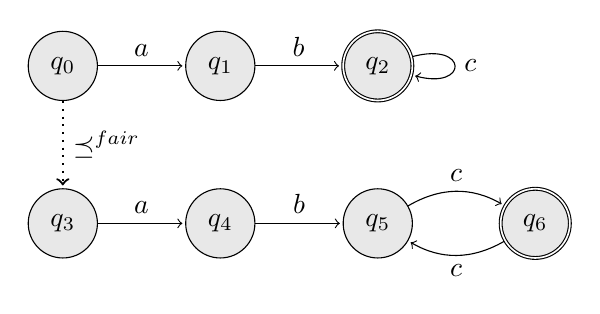
\begin{tikzpicture}[shorten >=1pt,node distance=2cm,auto]
  \tikzstyle{every state}=[fill={rgb:black,1;white,10}]
  \node[state] (q_0) {$q_0$};
  \node[state] (q_1) [right of=q_0]  {$q_1$};
  \node[state,accepting] (q_2) [right of=q_1]  {$q_2$};
  \node[state] (q_3) [below of=q_0] {$q_3$};
  \node[state] (q_4) [right of=q_3]  {$q_4$};
  \node[state] (q_5) [right of=q_4]  {$q_5$};
  \node[state,accepting] (q_6) [right of=q_5]  {$q_6$};
  \path[->]
  (q_0) edge node {$a$} (q_1)
  (q_1) edge node {$b$} (q_2)
  (q_2) edge [loop right] node {$c$} (q_2)
  (q_3) edge node {$a$} (q_4)
  (q_4) edge node {$b$} (q_5)
  (q_5) edge [bend left] node {$c$} (q_6)
  (q_6) edge [bend left] node {$c$} (q_5)
  ;
  \path[->,dotted,thick] (q_0) edge node {$\preceq^{fair}$} (q_3);
\end{tikzpicture}
\end{figure}
\end{frame}

%===============================================================================
\begin{frame}
\frametitle{New preorders}
The \textbf{context} of a word:
\begin{figure}[h]
\centering
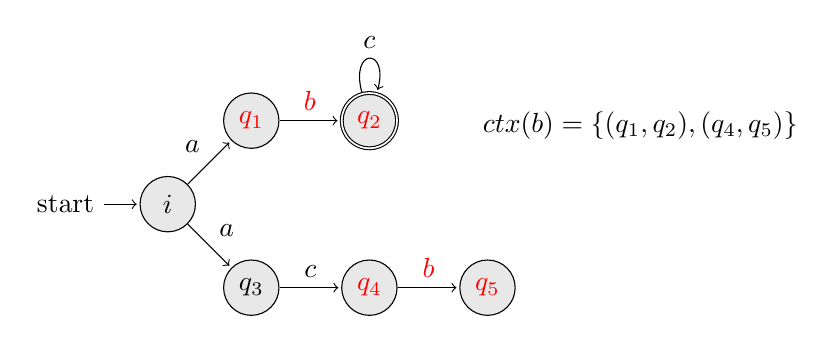
\begin{tikzpicture}[shorten >=1pt,node distance=1.5cm,auto]
  \tikzstyle{every state}=[fill={rgb:black,1;white,10}]
  \node[state,initial,inner sep=1pt,minimum size=20pt] (q_0) {$i$};
  \node[state,inner sep=1pt,minimum size=20pt] (q_1) [above right of=q_0]  {\textcolor{red}{$q_1$}};
  \node[state, accepting,inner sep=1pt,minimum size=20pt] (q_2) [right of=q_1]  {\textcolor{red}{$q_2$}};
  \node[state,inner sep=1pt,minimum size=20pt] (q_3) [below right of=q_0]  {$q_3$};
  \node[state,inner sep=1pt,minimum size=20pt] (q_4) [right of=q_3]  {\textcolor{red}{$q_4$}};
  \node[state,inner sep=1pt,minimum size=20pt] (q_5) [right of=q_4]  {\textcolor{red}{$q_5$}};
  \path[->]
  (q_0) edge node {$a$} (q_1)
  (q_1) edge node {\textcolor{red}{$b$}} (q_2)
  (q_2) edge [loop above] node {$c$} (q_2)
  (q_0) edge node {$a$} (q_3)
  (q_3) edge node {$c$} (q_4)
  (q_4) edge node {\textcolor{red}{$b$}} (q_5)
  ;
  \draw (6,1) node {$ctx(b) = \{(q_1,q_2), (q_4,q_5)\}$};
\end{tikzpicture}
\end{figure}
Generalization using \textbf{pairs} of states:
\begin{itemize}
\Large\item $\sqsubseteq_{\mathcal{B}}^1$
\item \Large$\sqsubseteq_{\mathcal{B}}^2$
\end{itemize}
\end{frame}


%===============================================================================
\begin{frame}
\frametitle{My work}
\begin{itemize}
\item Proved a list of requirements related to \textbf{computability} and \textbf{completeness}
    \begin{enumerate}
    \item computability
    \item right-monotonicity ($u \leq v \Longrightarrow uw \leq vw$)
    \item being a well-quasiorder (for each infinite sequence $\{x_i\}_{i \in \mathbb{N}}$, $\exists i,j: i < j \; \wedge \; x_i \leq x_j$)
    \item $\rho_{\leq_1 \times \leq_2}(I_{L_2}) = I_{L_2}$
    \end{enumerate}
\item Identified which pairs are suitable for the framework
\[ \sqsubseteq_{\mathcal{B}}^1, \sqsubseteq_{\mathcal{B}}^2 \]
\[ \sqsubseteq_{\mathcal{B}}^{r}, \sqsubseteq_{\mathcal{B}}^2 \]
\[ \sqsubseteq_{\mathcal{B}}^{de,r}, \sqsubseteq_{\mathcal{B}}^2 \]
\[ \sqsubseteq_{\mathcal{B}}^{fair,r}, \sqsubseteq_{\mathcal{B}}^2 \]
\end{itemize}
\end{frame}

%===============================================================================
\begin{frame}
\frametitle{Other considered simulations}
\begin{itemize}
\item $K$-lookahead simulations
\item Trace inclusions
\item ``$K$-delayed'' simulations
\end{itemize}
\pause
Problems related to \textbf{transitivity} and \textbf{completeness}.
\end{frame}

%===============================================================================
\begin{frame}
\frametitle{Taxonomy of the preorders}

\begin{figure}[h]
\centering
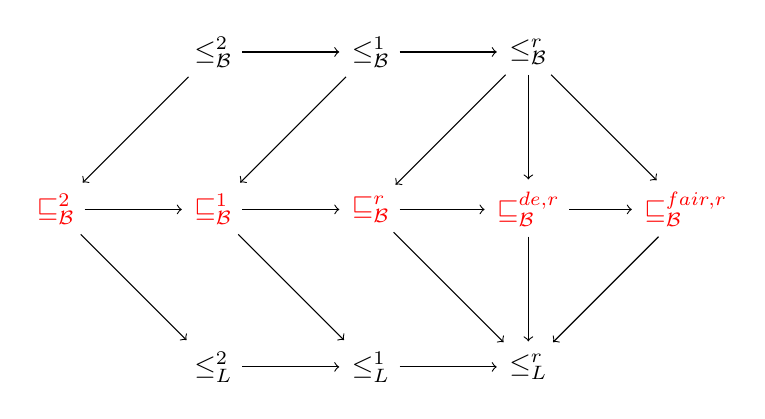
\begin{tikzpicture}[shorten >=1pt,node distance=2cm,auto]
  \tikzstyle{every state}=[fill={rgb:black,1;white,10}]
  \node (0) {$\leq^2_{\mathcal{B}}$};
  \node (1) [right of=0]{$\leq^1_{\mathcal{B}}$};
  \node (2) [right of=1]{$\leq^r_{\mathcal{B}}$};

  \node (4) [below of=0]{\textcolor{red}{$\sqsubseteq_{\mathcal{B}}^1$}};
  \node (3) [left of=4]{\textcolor{red}{$\sqsubseteq_{\mathcal{B}}^2$}};
  \node (5) [right of=4]{\textcolor{red}{$\sqsubseteq_{\mathcal{B}}^r$}};
  \node (6) [right of=5]{\textcolor{red}{$\sqsubseteq_{\mathcal{B}}^{de,r}$}};
  \node (7) [right of=6]{\textcolor{red}{$\sqsubseteq_{\mathcal{B}}^{fair,r}$}};

  \node (8) [below of=4] {$\leq^2_{L}$};
  \node (9)  [right of=8]{$\leq^1_{L}$};
  \node (10) [right of=9]{$\leq^r_{L}$};
  \path[->]
  (0) edge node {} (1)
  (0) edge node {} (3)
  (1) edge node {} (2)
  (1) edge node {} (4)
  (2) edge node {} (5)
  (2) edge node {} (6)
  (2) edge node {} (7)
  (3) edge node {} (4)
  (4) edge node {} (5)
  (5) edge node {} (6)
  (4) edge node {} (9)
  (3) edge node {} (8)
  (5) edge node {} (10)
  (6) edge node {} (10)
  (7) edge node {} (10)
  (6) edge node {} (7)
  (8) edge node {} (9)
  (9) edge node {} (10)
  ;
\end{tikzpicture}
\end{figure}
\end{frame}


%===============================================================================
\begin{frame}
\frametitle{Why bother?}
Simulations and the language inclusion problem:
\begin{itemize}
% nfa
\pause
\item \textbf{2010}: Abdulla, P.A. et al. \emph{When simulation meets antichains.}
% buchi
\pause
\item \textbf{2011}: Abdulla, P.A. et al. \emph{Advanced Ramsey-based B{\"u}chi automata inclusion testing.}
% nfa
\pause
\item \textbf{2013}: Bonchi, F. and Pous, D. \emph{Checking NFA equivalence with bisimulations up to congruence.}
% buchi
\pause
\item \textbf{2017}: Mayr, R. and Clemente, L. \emph{
Efficient reduction of nondeterministic automata with application to language inclusion testing.  }
\end{itemize}
\end{frame}

%===============================================================================
\begin{frame}
\frametitle{What's next}
\begin{figure}[h]
    \centering
    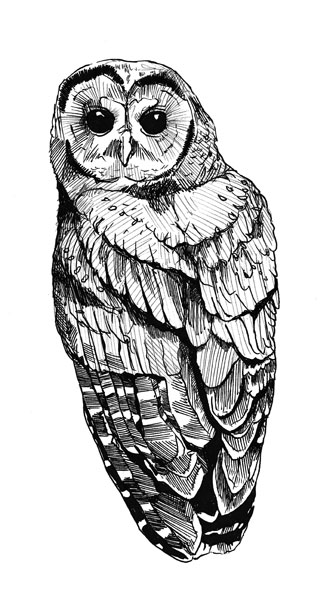
\includegraphics[width=0.3\textwidth]{../img/owl.jpg}
\end{figure}
\end{frame}

%===============================================================================
\begin{frame}
\begin{center}
\Huge Thanks for your attention
\end{center}
\end{frame}

%===============================================================================
% \begin{frame}
% \Huge{\centerline{Thanks for your attention}}
% \end{frame}


% \begin{frame}[allowframebreaks]
%         \frametitle{References}
%         \bibliographystyle{amsalpha}
%         \bibliography{../support/bibliography.bib}
% \end{frame}

\end{document}
